
%%%%%%%%%%%%%%%%%%%% file CSMC_MUME_LaTeX_Template.tex %%%%%%%%%%%%%%%%%%%%%
%
% This is the LaTeX source for the instructions to authors using
% the LaTeX document class 'llncs.cls' for contributions to
% the Journal of Creative Music Systems.
% Copyright: http://www.springer.com/lncs       Springer Heidelberg 2006/05/04
%
% It may be used as a template for your own input - copy it
% to a new file with a new name and use it as the basis
% for your article.
%
% NB: the document class 'llncs' has its own and detailed documentation, see
% ftp://ftp.springer.de/data/pubftp/pub/tex/latex/llncs/latex2e/llncsdoc.pdf
%
%%%%%%%%%%%%%%%%%%%%%%%%%%%%%%%%%%%%%%%%%%%%%%%%%%%%%%%%%%%%%%%%%%%

\documentclass[runningheads,a4paper]{llncs}

\usepackage{amssymb}
\setcounter{tocdepth}{3}
\usepackage{graphicx}
\usepackage{url}
\usepackage{apacite}
%added 
\usepackage[inline]{enumitem}    
\usepackage{subcaption}
\usepackage{caption}
\usepackage{threeparttable} %annotations for table
\usepackage{csquotes}


\newcommand{\keywords}[1]{\par\addvspace\baselineskip
\noindent\keywordname\enspace\ignorespaces#1}

\pagestyle{headings}

\begin{document}

\mainmatter  

\title{Percussive Sound Generation with Virtual Listeners and Modular Synthesizers}

% a short form should be given in case it is too long for the running head
\titlerunning{Virtual Percussive Sound Generation}

% the name(s) of the author(s) follow(s) next
\author{Amir Salimi \and Abram Hindle}

\authorrunning{Amir Salimi and Abram Hindle }

% the affiliations are given next; don't give your e-mail address
% unless you accept that it will be published
\institute{Department of Computing Science\\ University of Alberta \\ \email{asalimi@ualberta.ca}}

% intro, 1 page
% background and methodology 2 pages
% implementation 
% results 2.5
\maketitle

\begin{abstract}
Digital sound artists often require a variety of percussive samples for their music. For more than two decades research involving digital synthesis, heuristic search, and neural networks has been used for the generation of novel sounds. Our goal is to generate one-shot percussive samples by leveraging modern AI technologies alongside scalable signal generation methods. We centered our approach around the combination of two central components: \begin {enumerate*} [label=(\roman*)] \item a \emph{virtual ear} capable of evaluating the proximity of unheard sounds to  and \item a dynamic \emph{virtual synthesizer} with a rich set of tractable parameters\end{enumerate*}. We present a generative pipeline that utilizes robust digital signal processing methods guided by supervised learning towards the generation of one-shot percussive sounds. We present our findings and measurements of the various approaches taken. Advantages, shortcomings and practicality of the employed methodologies are demonstrated. We share our curated dataset of sounds and codebase\footnote{\url{https://github.com/imilas/Synths_Stacks_Search}} which can be used for its further expansion.
\keywords{Automatic Synthesizer design. Machine Listening. Sound Analysis. Novelty and Originality}
\end{abstract}

\section{Preamble}
\subsection{Drums and Percussion}
Drums are a subcategory of percussive instruments. Drum sounds such as kick and snare are two of the most universally recognized examples of percussion~\cite{barry2005drum}. Almost any object which is struck to produce noise can be referred to as a drum~\cite{latham2002oxford}. The term \enquote{Percussion} often encompasses all drums and may include the additional instruments which may be rubbed, plucked, blown, etc; A more strict definition of percussion can be used interchangeably with drums~\cite{latham2002oxford}. We adapt this strict definition for this work as our concern is not the delineation between the two overlapping concepts, but with extraction and creation of novel sounds with characteristics shared between the two. As a result, we often use the terms \enquote{drum} and \enquote{percussion} interchangeably.

\subsection{Motivation and Goals}
Digital recordings of novel, one-shot\footnote{A single hit on the drum that captures its capabilities} drum sounds are not easy or cheap to find. Our goal here is to create a new, virtual source of novel drum sounds, which could then be used in electronic music compositions.

By relying on recordings of \textit{real life} drum sounds, we are limited by what instruments exist in the real world and whether or not we have access to clean, one-shot recordings. Our hypothesis is that the virtualization of sound generation can alleviate these material limitations. 

 \begin{figure}[t!]
    \begin{center}
    \textbf{Pipeline Design}
    \makebox[\textwidth]{
    \fbox{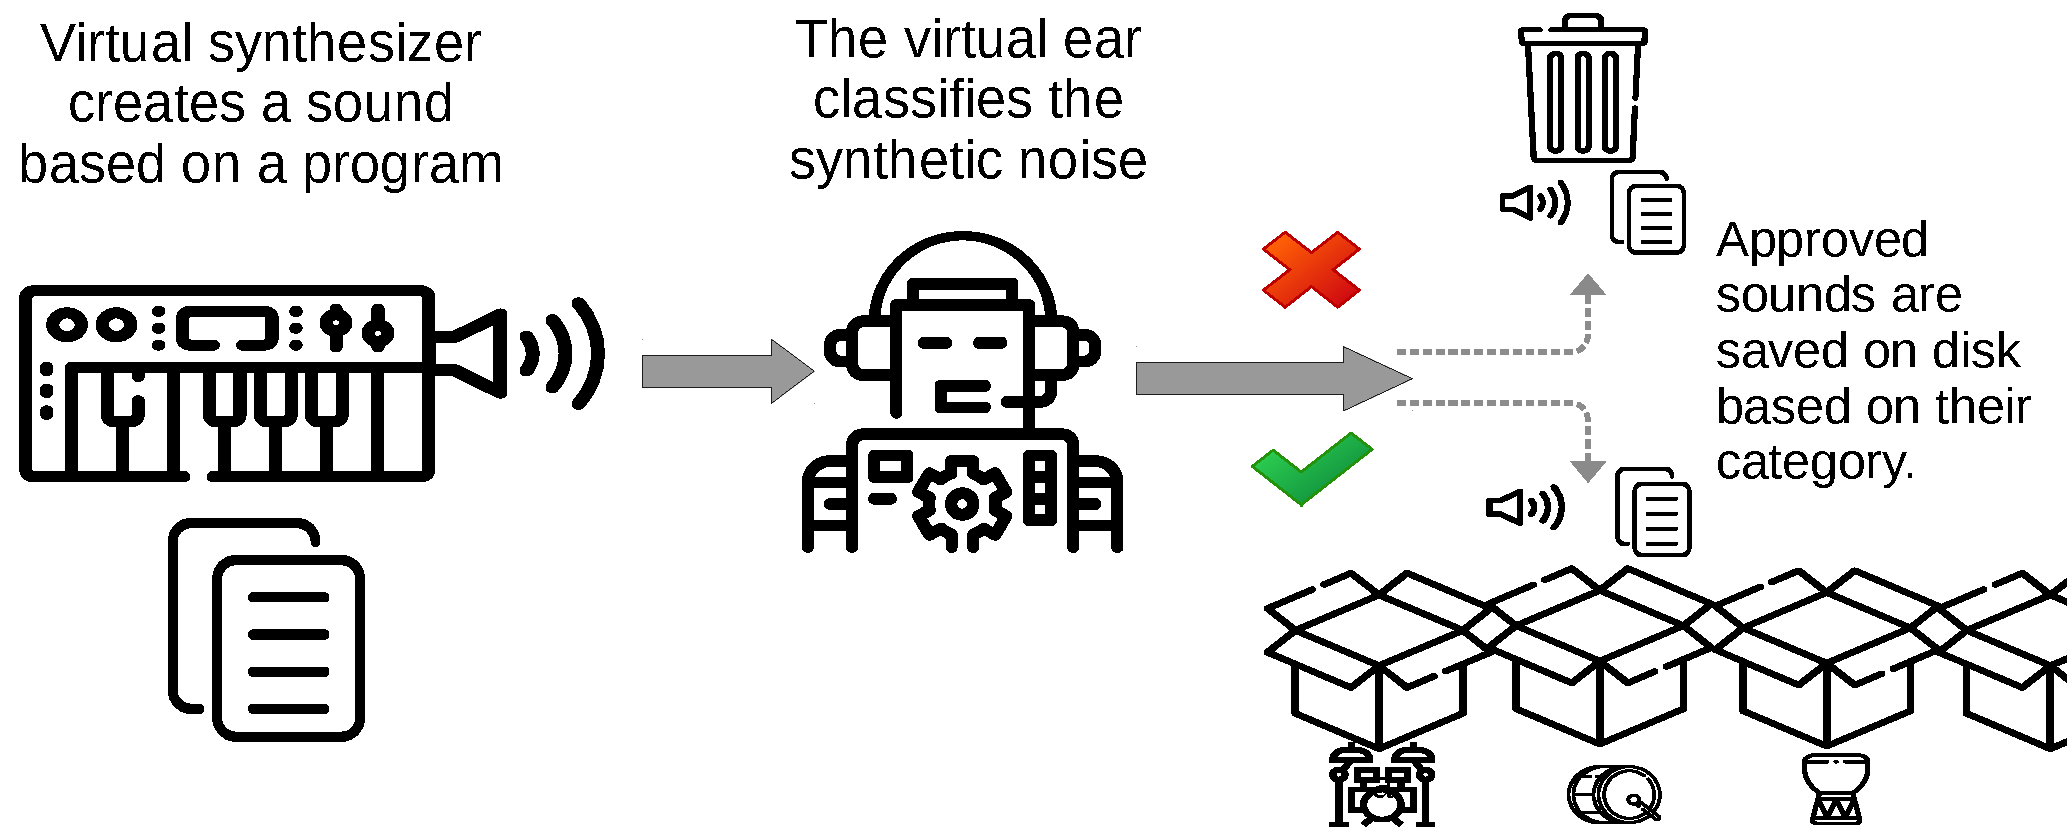
\includegraphics[width=1.1\linewidth]{images/pipeline.pdf}}}
    \end{center}
    \caption{A blueprint of our desired pipeline which allows each component to be implemented in a number of ways. Our implementations of this pipeline allow for easy parallelization when needed. 
    }
\label{fig:pipeline_outline}
\end{figure}



\subsection{Related Works}
\label{related_works}
\begin{center}
\begin{table}[h]
\resizebox{\linewidth}{!}{\begin{tabular}{|c c c c|} 
\hline
Work & Feature extraction & Synthesis & Specilization & \hline
Oord 2017 & CNN & CNN &Speech& \hline
Yee-King 2018 & LSTM on Paremters & DSP & Synth Pads & \hline
Aouameur 2019 & Latent layer& Decoding of Latent Layers & Percussion & \hline
Ramires 2020 & Latent layer & FeedForward Network & Percussion & \hline
Yamamoto 2020 & GAN & GAN & Speech & \hline
\end{tabular}}
\caption{Quick reference of recent related works}
\end{table}
\label{table:recent_works}
\end{center}
Numerous deep, neural network models have been proposed and utilized for the purpose of signal generation in recent years. WaveGans and WaveNet have been subject to significant improvements and experiments since their proposal~\cite{nsynth2017,yamamoto2020parallel,oord2017parallel}. Most relevant to us are recent works by Aoumaeur et al. in which variational AutoEncoders (VAE's) have been utilized for generation of percussive samples~\cite{aouameur2019neural}; As well as Ramires et al's work in generation of percussive sounds by guiding the output of a feedforward neural network via a small set of latent features~\cite{ramires2020neural}. 
Automatic programming of virtual synthesizers has long been a topic of interest. In early 2000s, Interactive Genetic Algorithms (IGA's) were utilized for the generation of new sounds with various sound-engines~\cite{johnson1999exploring,dahlstedt2001creating}. More recent work by Yee-King et al.~\cite{yee2018automatic} used Long short-Term Memory (LSTM) models and genetic algorithms to find the exact parameters used to create a group of sounds. The sounds approximated were made by the same virtual synthesizer, not an external source; making the eventual replication certain even with random search. Since this work appears more focused on pads and textures rather than drums, feature matching appears to not be concerned with the envelope of the sounds but rather the frequency content within arbitrary time windows. Yet another recent work by Esling et al. used a large dataset of over 10,000 presets for a commercial VST synthesizer to learn a latent parameter space which can be sampled for creation of new audio~\cite{esling2019universal}. As stated before, our work explores the rapid approximation of percussion sounds with no previous knowledge about the sonic capabilities of our virtual synthesizer, exploring the actual parameter space rather than its latent representation.

\subsection{Our Approach}
To virtually create novel drum sounds, we need a tractable, generative source of audio; One that deterministically produces audio based on a set of instructions. Additionally, we need a method of evaluation to help us determine which sounds resemble drums and are worth keeping. To enable heuristic search, we would like to know what instructions caused our audio source to make the sounds we liked. Given these two components capable of \textit{generation} and \textit{evaluation} of sounds, we build a generative pipeline of audio as depicted in figure~\ref{fig:pipeline_outline}. The success of this pipeline is dependent on the characteristics of the components responsible for the generation and evaluation of the sounds. We call these two components the \emph{virtual synthesizer} and \emph{virtual ear} respectively.  
\begin{figure}[t!]
    \begin{center}
    \textbf{Data Overview}
    \makebox[\textwidth]{
    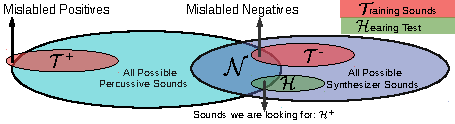
\includegraphics[width=1.1\linewidth]{images/venn_data.pdf}}
    \end{center}
    \caption{ 
    Scales are symbolic (True scales are not measurable and/or subjective). Our positive samples, $\mathcal{T^{+}}$, is a small fraction of a wide variety of percussive sounds that are conceivable. The size of $\mathcal{T^{-}}$ can be set to any number(we can generate any number of random samples), but we prefer to keep it no larger than  $\mathcal{T^{+}}$. $\mathcal{H}$ is a series of sounds sent to the ear for classification. The ideal ear will detect  $\mathcal{H^{+}}$, the overlap of $\mathcal{H}$ and $\mathcal{N}$, with high precision and recall. 
    }
\label{fig:ven_data}
\end{figure}


\subsection{Virtual Synthesizer Design}
Sound is product of physical disturbances, causing vibrations in our mediums. Vibrations are perpetuated through air as part of an expanding, spherical front ~\cite{cook1999chap4}. A sound wave can be viewed as the result of a function which governs amplitude through time, where time and amplitude exist in continuous dimensions. Waves can be approximated via a series of samples, associating time steps to a discrete range of amplitude values.~\textit{Digital synthesis} of audio is the process of creating these discrete values.
Unlike the majority of the works mentioned in Section~\ref{related_works}, we do not employ probabilistic models for the synthesizer component. Our decision is based on the following factors:
\begin{itemize}
    \item \textit{Interpretability and Expansion}:
    \item \textit{Novelty and Creativity}: Given large sets of examples, generative models such as VAEs and GANS have proven capable of generating samples similar to the exemplars. we are not aiming for perfect imitations, rather, we want to work with the limitations of any tractable sound source to create its novel approximations of a given sound category.     
    \item \textit{Efficiency}: 

\end{itemize}

\begin{figure*}[htbp]
\label{fig_example_sine}
\centering
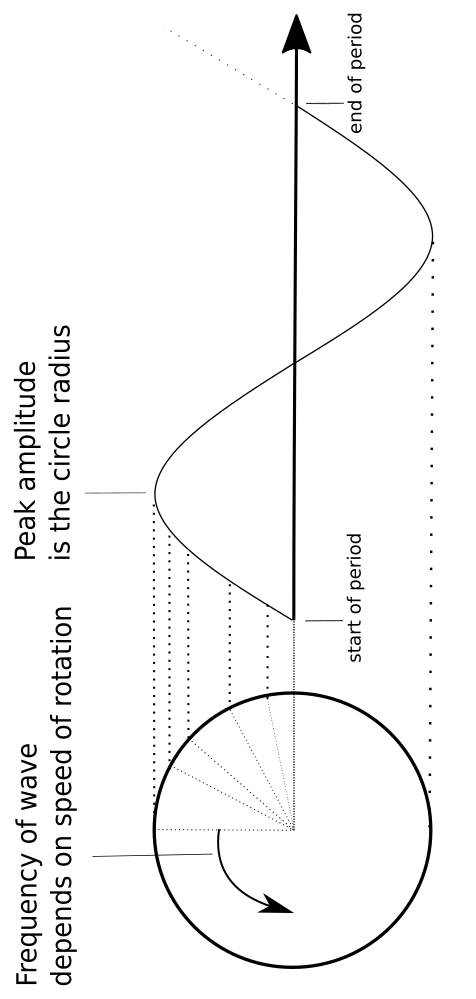
\includegraphics[width=0.45\linewidth,angle =-90 ]{images/periodic_function.png}
\caption{A computer can simulate waveforms by utilizing periodic functions. Digital waveforms are discrete approximations of analogue waves. \cite{mitchell2009basicsynthChap5} }
\end{figure*}

Evaluation of a periodic function such as sine or cosine is the simplest form of software audio generation~\cite{mitchell2009basicsynthChap5}. This generative system is called an \textit{oscillator}. The combination and modification of oscillators are the building blocks of digital signal processing (DSP). Most sounds from the natural environment, and its flora and fauna are more complex than the output of a single oscillator. However, with careful programming, DSP techniques can be used to replicate almost any sound, which is why they have powered commercial digital synthesizers for over half a century ~\cite{jenkins2019analog}. Another advantage to using DSP for sound generation is that the synthesizers we build using these functions are tractable: the output is determined by the input and reproducible. This makes the evaluation of a set of inputs (or parameters) to our synthesizers  simpler compared to the evaluation of synthesizers that utilize probabilistic models.
 
\subsection{How Can a Computer Evaluate Sounds?}
Automatic evaluation of sounds is an essential component of our work: A thorough manual evaluation of outputs is not possible when hundreds can be created in a second. In our work, we find simple features such as frequency content (high pitch vs low pitch), length, and envelope (change in loudness, how fast the sounds reaches its maximum loudness and fades away) to be powerful for the categorization of drum sounds. Later on we will discuss our algorithms for extraction of these and other features in~\ref{implementation}. We will also discuss how these extracted features were used to train models that can automatically categorize new sounds.  

\section{Implementation}
We conceptualized a general pipeline for approximation of sounds: A synthesizer creates random noise while a virtual ear rapidly evaluates the outputs and outputs a score which is used for the separation of undesired outputs from desired ones. This approach assumes that a fraction of the randomly generated sounds can be substituted for percussion and that the synthetic ear will assign higher evaluation scores to this subset. 
\begin{itemize}
    \item \textit{Virtual Synthesizer}: A flexible, deter\-min\-istic, and tract\-able gener\-ator which can create audio. 
    \item \textit{Virtual Ear}: An ear that returns an evaluation of an audio sample; estimating the effectiveness of an audio sample's fulfillment of a producers requirements. The ear's evaluation guides the generation process towards a desired path, making it a crucial component of our pipeline. 
\end{itemize}
We wish to leverage AI technologies, heuristic search, and DSP methods for the synthesis of novel audio. The work here is motivated by the idea of finding new, convenient methods for the expansion of a music producer's library of sounds. We demonstrate our work in combining machine listening and automatic synthesizer programming to find pieces of audio which can be used as drums. Using the generation of short, percussive audio samples as a starting point, this project is a proof of concept for a modular, generative pipeline of novel, one-shot audio samples. Design decisions were made such that this approach can be modified for creation of other, non-percussive sound-types. 
Instead of learning weights and parameters in an audio-generation neural network, we wish to generate, search, and tune synthesizers to produce percussion sounds.





\bibliographystyle{apacite}
\bibliography{CSMC_MUME_LaTeX_Template.bib}

\end{document}
